%% Creator: Inkscape inkscape 0.92.2, www.inkscape.org
%% PDF/EPS/PS + LaTeX output extension by Johan Engelen, 2010
%% Accompanies image file 'fle6.eps' (pdf, eps, ps)
%%
%% To include the image in your LaTeX document, write
%%   \input{<filename>.pdf_tex}
%%  instead of
%%   \includegraphics{<filename>.pdf}
%% To scale the image, write
%%   \def\svgwidth{<desired width>}
%%   \input{<filename>.pdf_tex}
%%  instead of
%%   \includegraphics[width=<desired width>]{<filename>.pdf}
%%
%% Images with a different path to the parent latex file can
%% be accessed with the `import' package (which may need to be
%% installed) using
%%   \usepackage{import}
%% in the preamble, and then including the image with
%%   \import{<path to file>}{<filename>.pdf_tex}
%% Alternatively, one can specify
%%   \graphicspath{{<path to file>/}}
%% 
%% For more information, please see info/svg-inkscape on CTAN:
%%   http://tug.ctan.org/tex-archive/info/svg-inkscape
%%
\begingroup%
  \makeatletter%
  \providecommand\color[2][]{%
    \errmessage{(Inkscape) Color is used for the text in Inkscape, but the package 'color.sty' is not loaded}%
    \renewcommand\color[2][]{}%
  }%
  \providecommand\transparent[1]{%
    \errmessage{(Inkscape) Transparency is used (non-zero) for the text in Inkscape, but the package 'transparent.sty' is not loaded}%
    \renewcommand\transparent[1]{}%
  }%
  \providecommand\rotatebox[2]{#2}%
  \ifx\svgwidth\undefined%
    \setlength{\unitlength}{480.11991bp}%
    \ifx\svgscale\undefined%
      \relax%
    \else%
      \setlength{\unitlength}{\unitlength * \real{\svgscale}}%
    \fi%
  \else%
    \setlength{\unitlength}{\svgwidth}%
  \fi%
  \global\let\svgwidth\undefined%
  \global\let\svgscale\undefined%
  \makeatother%
  \begin{picture}(1,0.73473343)%
    \put(0,0){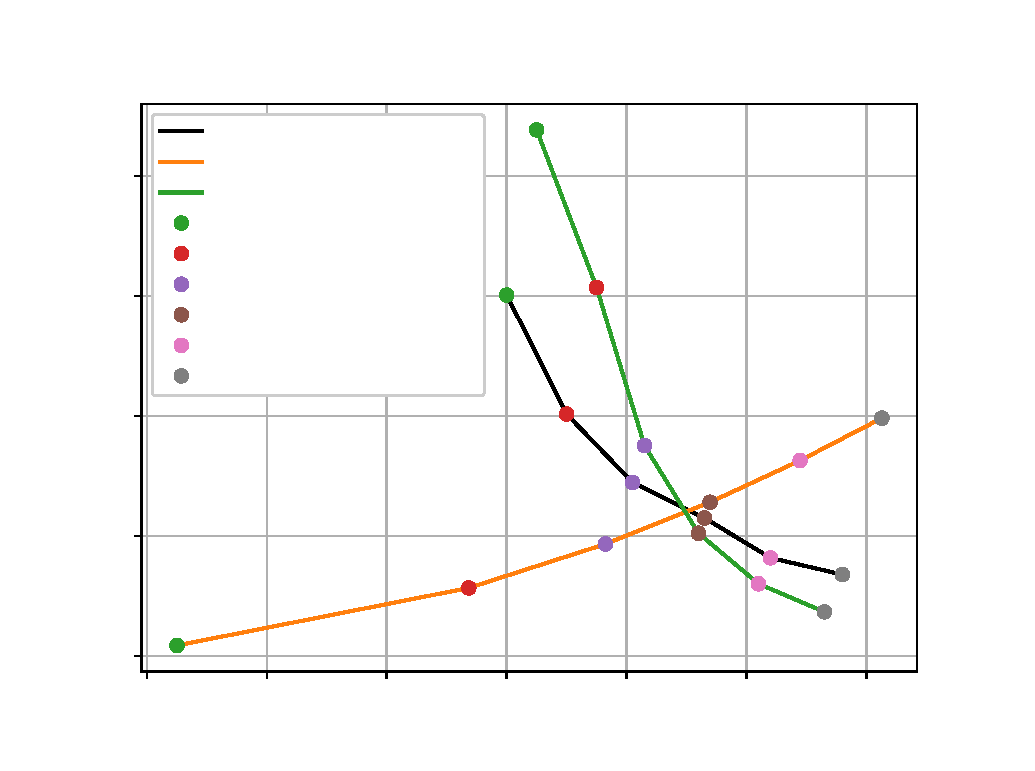
\includegraphics[width=\unitlength]{images_2ddl/fle6.eps}}%
    \put(0.12374434,0.05059935){\color[rgb]{0,0,0}\makebox(0,0)[lb]{\smash{6}}}%
    \put(0.24359106,0.05059935){\color[rgb]{0,0,0}\makebox(0,0)[lb]{\smash{8}}}%
    \put(0.35681486,0.05059935){\color[rgb]{0,0,0}\makebox(0,0)[lb]{\smash{10}}}%
    \put(0.47665992,0.05059935){\color[rgb]{0,0,0}\makebox(0,0)[lb]{\smash{12}}}%
    \put(0.59650706,0.05059935){\color[rgb]{0,0,0}\makebox(0,0)[lb]{\smash{14}}}%
    \put(0.7163542,0.05059935){\color[rgb]{0,0,0}\makebox(0,0)[lb]{\smash{16}}}%
    \put(0.83620134,0.05059935){\color[rgb]{0,0,0}\makebox(0,0)[lb]{\smash{18}}}%
    \put(0.07732198,0.08822412){\color[rgb]{0,0,0}\makebox(0,0)[lb]{\smash{0.5}}}%
    \put(0.07732198,0.20819831){\color[rgb]{0,0,0}\makebox(0,0)[lb]{\smash{1.0}}}%
    \put(0.07732198,0.3281725){\color[rgb]{0,0,0}\makebox(0,0)[lb]{\smash{1.5}}}%
    \put(0.07732198,0.44814878){\color[rgb]{0,0,0}\makebox(0,0)[lb]{\smash{2.0}}}%
    \put(0.07732198,0.56812297){\color[rgb]{0,0,0}\makebox(0,0)[lb]{\smash{2.5}}}%
    \put(0.06407654,0.30713401){\color[rgb]{0,0,0}\rotatebox{90}{\makebox(0,0)[lb]{\smash{$H_{max} (m)$}}}}%
    \put(0.45665992,0.02){\color[rgb]{0,0,0}\makebox(0,0)[lb]{\smash{$r_1 (mm)$}}}%
    \put(0.2020956,0.61339708){\color[rgb]{0,0,0}\makebox(0,0)[lb]{\smash{\footnotesize flambement/écoulement}}}%
    \put(0.2020956,0.58283804){\color[rgb]{0,0,0}\makebox(0,0)[lb]{\smash{\small $\delta/R>0.1$}}}%
    \put(0.2020956,0.55227901){\color[rgb]{0,0,0}\makebox(0,0)[lb]{\smash{\footnotesize écrasement de section}}}%
    \put(0.2020956,0.52171998){\color[rgb]{0,0,0}\makebox(0,0)[lb]{\smash{$r_2=15 mm$}}}%
    \put(0.2020956,0.49116095){\color[rgb]{0,0,0}\makebox(0,0)[lb]{\smash{$r_2=16 mm$}}}%
    \put(0.2020956,0.46060192){\color[rgb]{0,0,0}\makebox(0,0)[lb]{\smash{$r_2=17 mm$}}}%
    \put(0.2020956,0.43004497){\color[rgb]{0,0,0}\makebox(0,0)[lb]{\smash{$r_2=18 mm$}}}%
    \put(0.2020956,0.39948594){\color[rgb]{0,0,0}\makebox(0,0)[lb]{\smash{$r_2=19 mm$}}}%
    \put(0.2020956,0.3689269){\color[rgb]{0,0,0}\makebox(0,0)[lb]{\smash{$r_2=20 mm$}}}%
  \end{picture}%
\endgroup%
